\section[Búsqueda Scopus]{Búsqueda Scopus}
\begin{frame}
    \frametitle{Tendencia Scopus}
    \begin{columns}
      \column{0.6\textwidth}
    \begin{itemize}
      \item \textbf{El número de publicaciones es reducido}, aunque presenta una tendencia creciente.
        \begin{itemize}
          \item Tampoco existen muchos conjuntos de datos con la altura de las personas etiquetada.
        \end{itemize}
      \item La tarea consiste en estimar medidas en escala absoluta (en metros).
        \begin{itemize}
          \item \textbf{Objetivo}: explotar ciertas invariantes geométricas.
        \end{itemize}
    \end{itemize}
    \column{0.4\textwidth}
    \begin{figure}
      \begin{center}
        
\includegraphics[width=\textwidth]{imagenes/chapter1/Scopus-Analyze-Year}
      \end{center}
      \caption{Tendencia de publicaciones en el campo según Scopus.}
    \end{figure}
  \end{columns}
  \vspace{-.2cm}
\end{frame}
\note{
  La metrología de vista única, como se mencionaba anteriormente, está captando cada vez más atención, véase la Figura de publicaciones relacionadas sacada de Scopus.
  La tendencia es positiva, aunque sean pocos los números de artículos publicados.
  Esto puede que esté relacionado con las dificultades del campo y la poca disponibilidad de datos etiquetados con alturas reales.
  %Hay varios factores que afectan a las estimaciones: problemas lumínicos, escenas con poca información geométrica o las distorsiones en la escena.
}
\section{Procedimiento}
\begin{frame}
  \frametitle{Descripción del procedimiento exacto de Zhu~\emph{et al.}}
  \begin{figure}[!ht]
  \begin{center}
      \includegraphics[width=\textwidth]{imagenes/appendix/teaser.pdf}
  \end{center}
  \caption{Descripción del procedimiento de metrología monocular sacada de Zhu~\emph{et al.}\footcite{SVMIW}}
  \end{figure}
\end{frame}

\begin{frame}
  \frametitle{Ecuaciones de proyección}
    \begin{enumerate}
      \item Utilizando geometría proyectiva obtenemos las siguientes ecuaciones:
    \end{enumerate}
    \vspace{.5cm}
      \begin{equation}
          v_t = \frac{(f\, cos\theta + v_c\, sin\theta)\,h_{obj} + (-f\, sin\theta + v_c\, cos\theta)z - f\,h_{cam}}{h_{obj}tan\theta + z\,cos\theta}
      \end{equation}
      \begin{equation}
        v_b = \frac{-f\,sin\theta z + v_c cos\theta z - f\,h_{cam}}{z\, cos\theta}
      \end{equation}
    \begin{enumerate}
      \item Donde ``$v_t$'' y ``$v_b$'' son la parte superior e inferior de la persona en la imagen.
    \end{enumerate}
    \footcitetext{SVMIW}
\end{frame}

\section{Ratio cruzado}
\begin{frame}
  \frametitle{Ejemplo de ratio cruzado\footcite{VisionBookMIT}}
\begin{figure}[!ht]
  \centering
  \subfloat{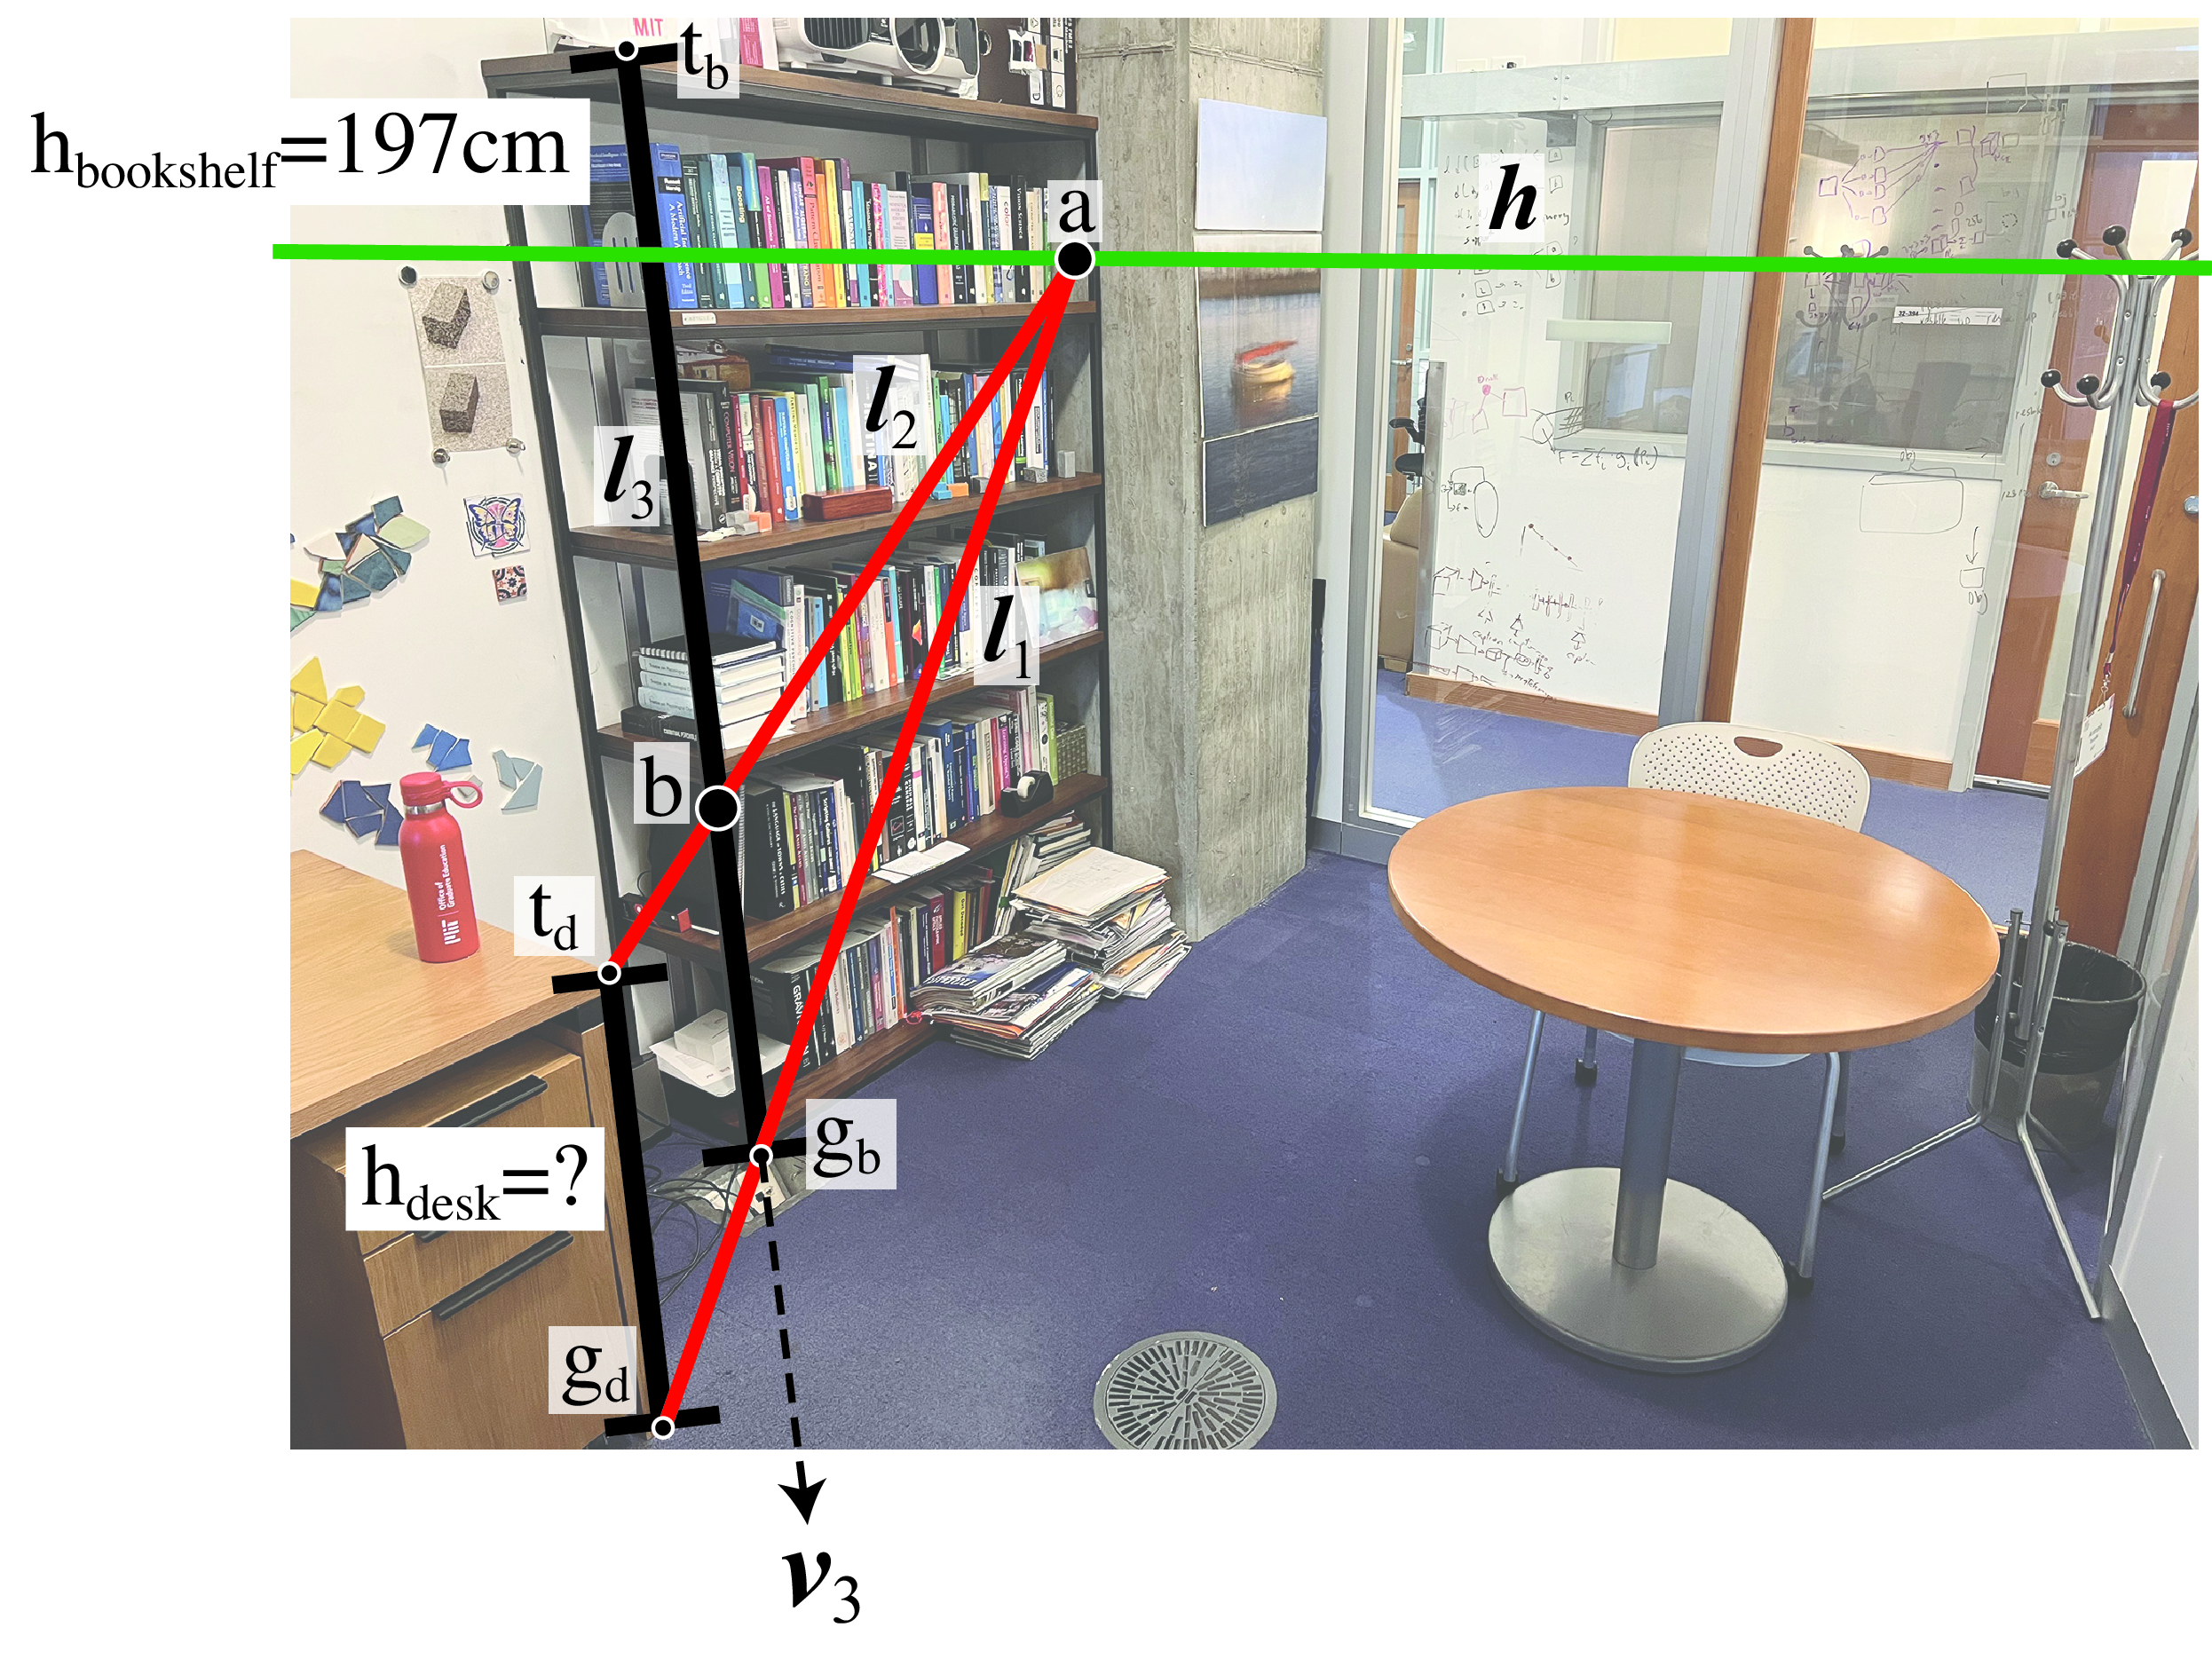
\includegraphics[width=.5\textwidth]{imagenes/appendix/office_measuring_desk.png}}\\
\end{figure}
\end{frame}

\section{Visualización de predicciones erróneas}
\begin{frame}
  \frametitle{Visualización de predicciones.}
\begin{figure}[!ht]
  \centering
  \subfloat{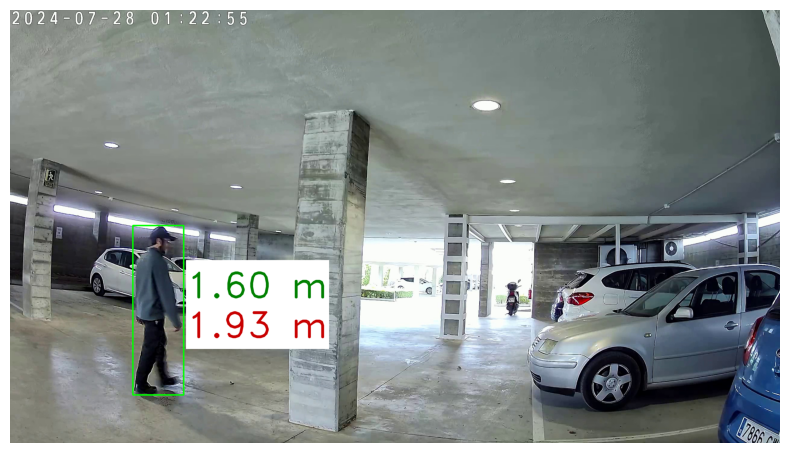
\includegraphics[width=0.5\textwidth]{imagenes/appendix/worst_fail_cam1_svmiw.png}}
  \subfloat{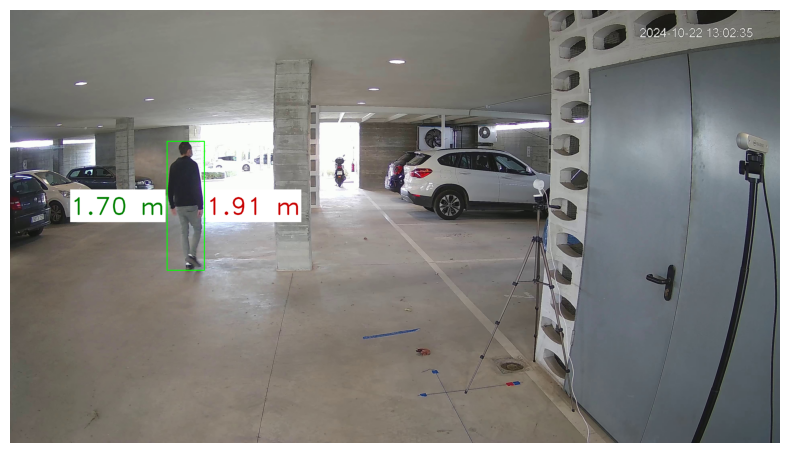
\includegraphics[width=0.5\textwidth]{imagenes/appendix/worst_fail_cam2_svmiw.png}}\\
\caption{Se observan las peores predicciones de las cámaras 1 y 2 con el método por aprendizaje.}
\end{figure}
\end{frame}

\begin{frame}
  \frametitle{Ejemplo de errores de consistencia.}
\begin{figure}[!ht]
  \centering
  \subfloat{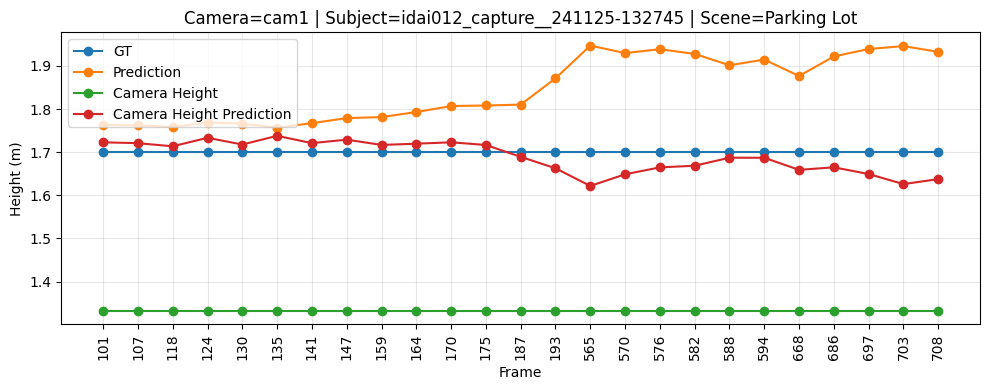
\includegraphics[width=1\textwidth]{imagenes/appendix/170-decrease-with-distance.png}}\\
\caption{Ejemplo de divergencia en la consistencia de la predicción al cambiar la distancia.}
\end{figure}
\end{frame}

\section{Distribución de datos}
\frametitle{Características de las cámaras simuladas}
\begin{frame}
  \begin{figure}[!htp]
  \begin{center}
    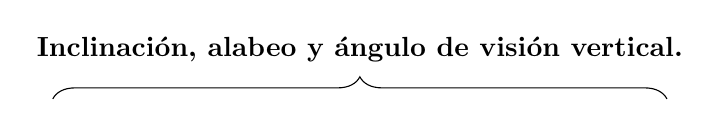
\begin{tikzpicture}[baseline]
        \draw[decorate,decoration={brace,amplitude=8pt}]
            (1.2cm,0) -- (9cm,0)
            node[midway,above=10pt] {\textbf{Inclinación, alabeo y ángulo de visión vertical.}};
    \end{tikzpicture}\\
    \subfloat{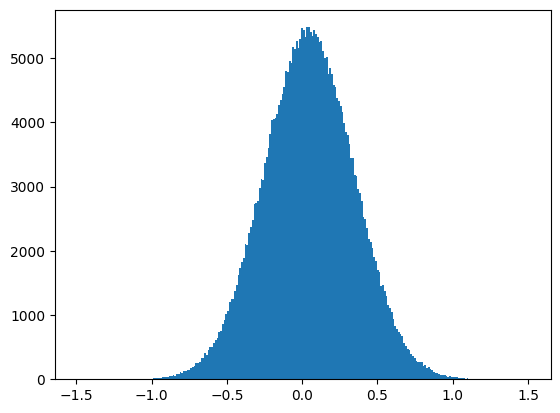
\includegraphics[width=0.35\textwidth]{imagenes/appendix/pitch_spec_dist.png}}
    \subfloat{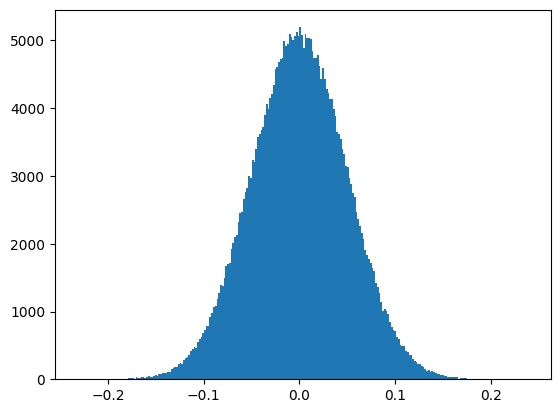
\includegraphics[width=0.35\textwidth]{imagenes/appendix/roll_spec_dist.png}}
    \subfloat{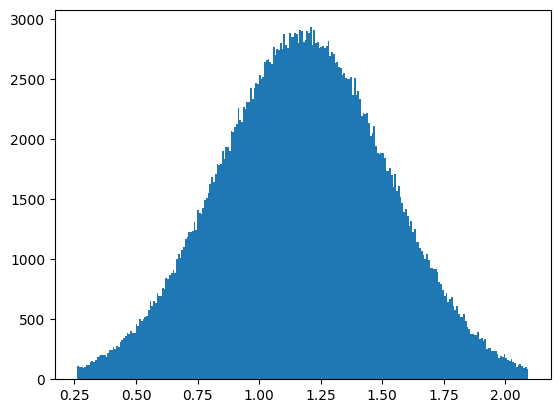
\includegraphics[width=0.35\textwidth]{imagenes/appendix/vfov_spec_dist.png}}
  \end{center}
  \caption[Visualización de la distribución de los ángulos de cámara utilizados por~\footcite{SPEC}.]{
    Visualización de la distribución de los ángulos de cámara utilizados por~\footcite{SPEC}.
  }
  \end{figure}
\end{frame}

\section{Entorno de desarrollo}
\begin{frame}
  \frametitle{Tecnologías utilizadas}
  \begin{table}[htp]
      \begin{tabular}{cccc}
        \begin{minipage}{.2\textwidth}
          
\includegraphics[width=\textwidth]{imagenes/appendix/tech/Python}
        \end{minipage}
                                  &
        \begin{minipage}{.2\textwidth}
          
\includegraphics[width=.65\textwidth]{imagenes/appendix/tech/d2}
        \end{minipage}
                                  &
        \begin{minipage}{.2\textwidth}
          
\includegraphics[width=\textwidth]{imagenes/appendix/tech/Pytorch}
        \end{minipage}
                                  &
        \begin{minipage}{.2\textwidth}
          
\includegraphics[width=.6\textwidth]{imagenes/appendix/tech/OpenCV}
        \end{minipage}
                                  \\
        \begin{minipage}{.2\textwidth}
          
\includegraphics[width=\textwidth]{imagenes/appendix/tech/Numpy}
        \end{minipage}
                                                        &
        \begin{minipage}{.2\textwidth}
          
\includegraphics[width=.9\textwidth]{imagenes/appendix/tech/Scikit}
        \end{minipage}
                                                        &
        \begin{minipage}{.2\textwidth}
          
\includegraphics[width=.9\textwidth]{imagenes/appendix/tech/Polars}
        \end{minipage}
        &
        \begin{minipage}{.2\textwidth}
          
\includegraphics[width=.55\textwidth]{imagenes/appendix/tech/pandas}
        \end{minipage} \\
                                                        &
        \begin{minipage}{.2\textwidth}
          
\includegraphics[width=.9\textwidth]{imagenes/appendix/tech/Nvidia}
        \end{minipage}
                                                        &
        \begin{minipage}{.2\textwidth}
          
\includegraphics[width=.9\textwidth]{imagenes/appendix/tech/Colab}
        \end{minipage}
                                                        &
                                                        \\
      \end{tabular}
  \end{table}
\end{frame}
